\chapter{Résultats expérimentaux}

\section{Le TbPc$_2$}
%\subsection{Présentation}
Nous avons vu, dans le chapitre premier, qu'un aimant moléculaire était en général composé de plusieurs centres magnétiques interagissant entre eux et que de cette interaction résultait un moment magnétique. Le Terbium double-decker, nommé ainsi par analogie aux avions du même nom, n’obéi pas à cette description. Il comporte un unique centre magnétique, l'ion terbium, pris en sandwich entre deux ligands, les ptalocyanines (cf Fig.\ref{TbPc2Imag}). Il présente néanmoins des propriétés magnétiques similaires aux aimants moléculaire à plusieurs centres avec cependant quelques particularités.

\begin{figure}
\centering 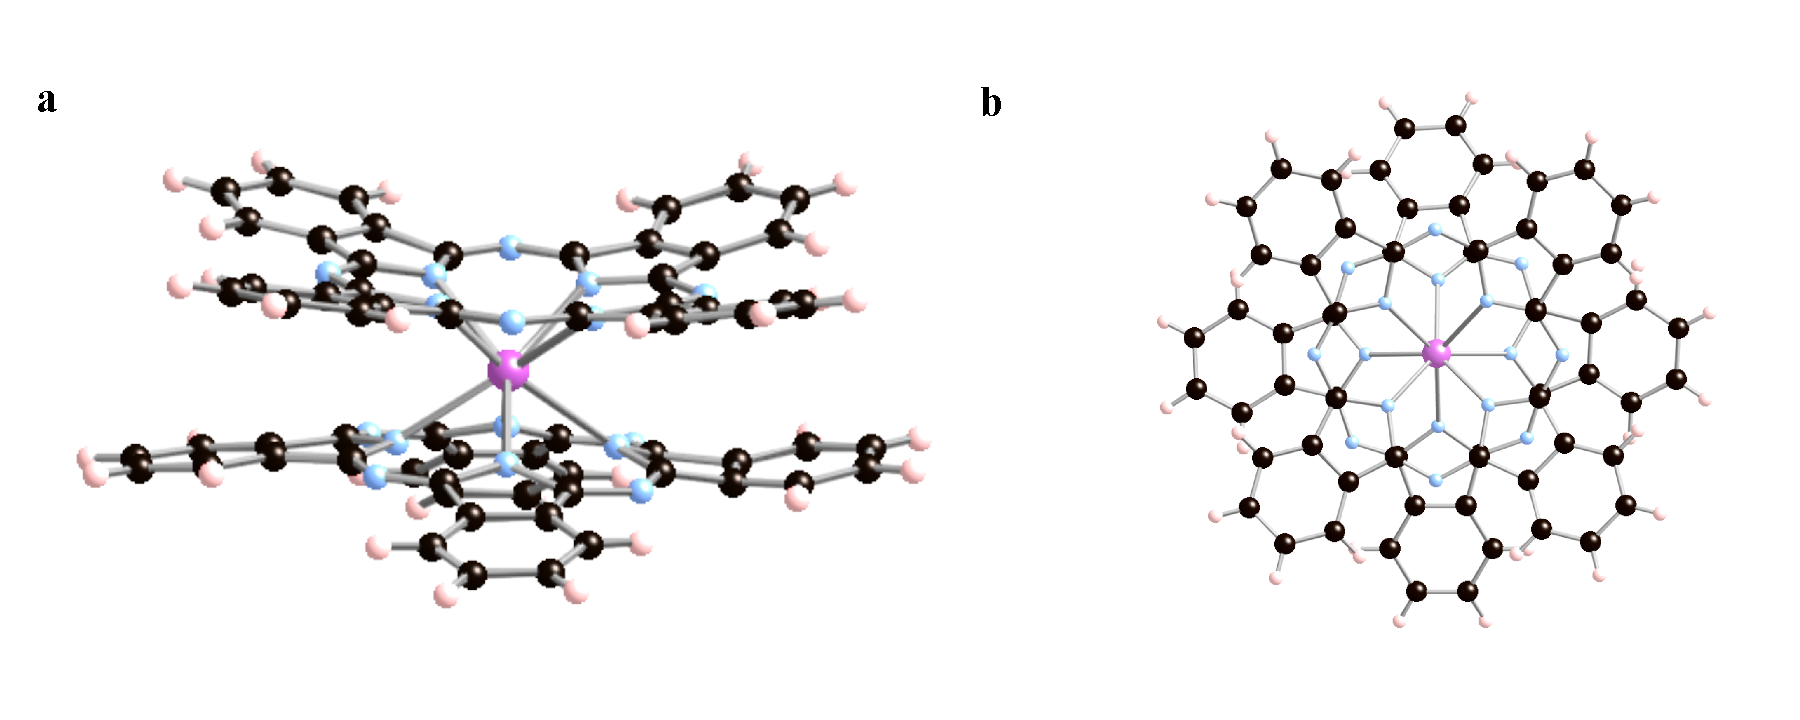
\includegraphics[scale=0.45]{Resultats/TbPc2Imag/TbPc2Imag.pdf} 
\caption{Vue d'artiste de la molécule de terbium double decker de côté~(\textbf{a}) et de dessus~(\textbf{b}). L'atome de terbium, ici en violet est pris en sandwich entre deux phtalocyanines, ces derniers étant orientés à $45\degres$ environs, l'un par rapport à l'autre.}
\label{TbPc2Imag}
\end{figure}





\subsection{Origine du moment magnétique}
Le moment magnétique du terbium double-decker est d\^u à un centre magnétique unique : l'ion Tb$^{3+}$. L'atome de Terbium appartient à la classe des lanthanide. Son magnétisme est porté par la couche $4f$ et résulte d'un fort couplage entre le moment de spin et le moment orbital. Du fait de cet interaction, le moment magnétique total de l'état fondamental est $J=6$ issue d'une contribution égale entre le moment magnétique angulaire $L=3$ et les moments magnétiques de spin des 6 électrons non appariés $S=3$. Le premier état excité $J=5$ est distant de $2900\,K$ et peut donc \^etre ignoré lorsque l'on s'intéresse aux propriété magnétique de la molécule.
 

\begin{figure}
\centering 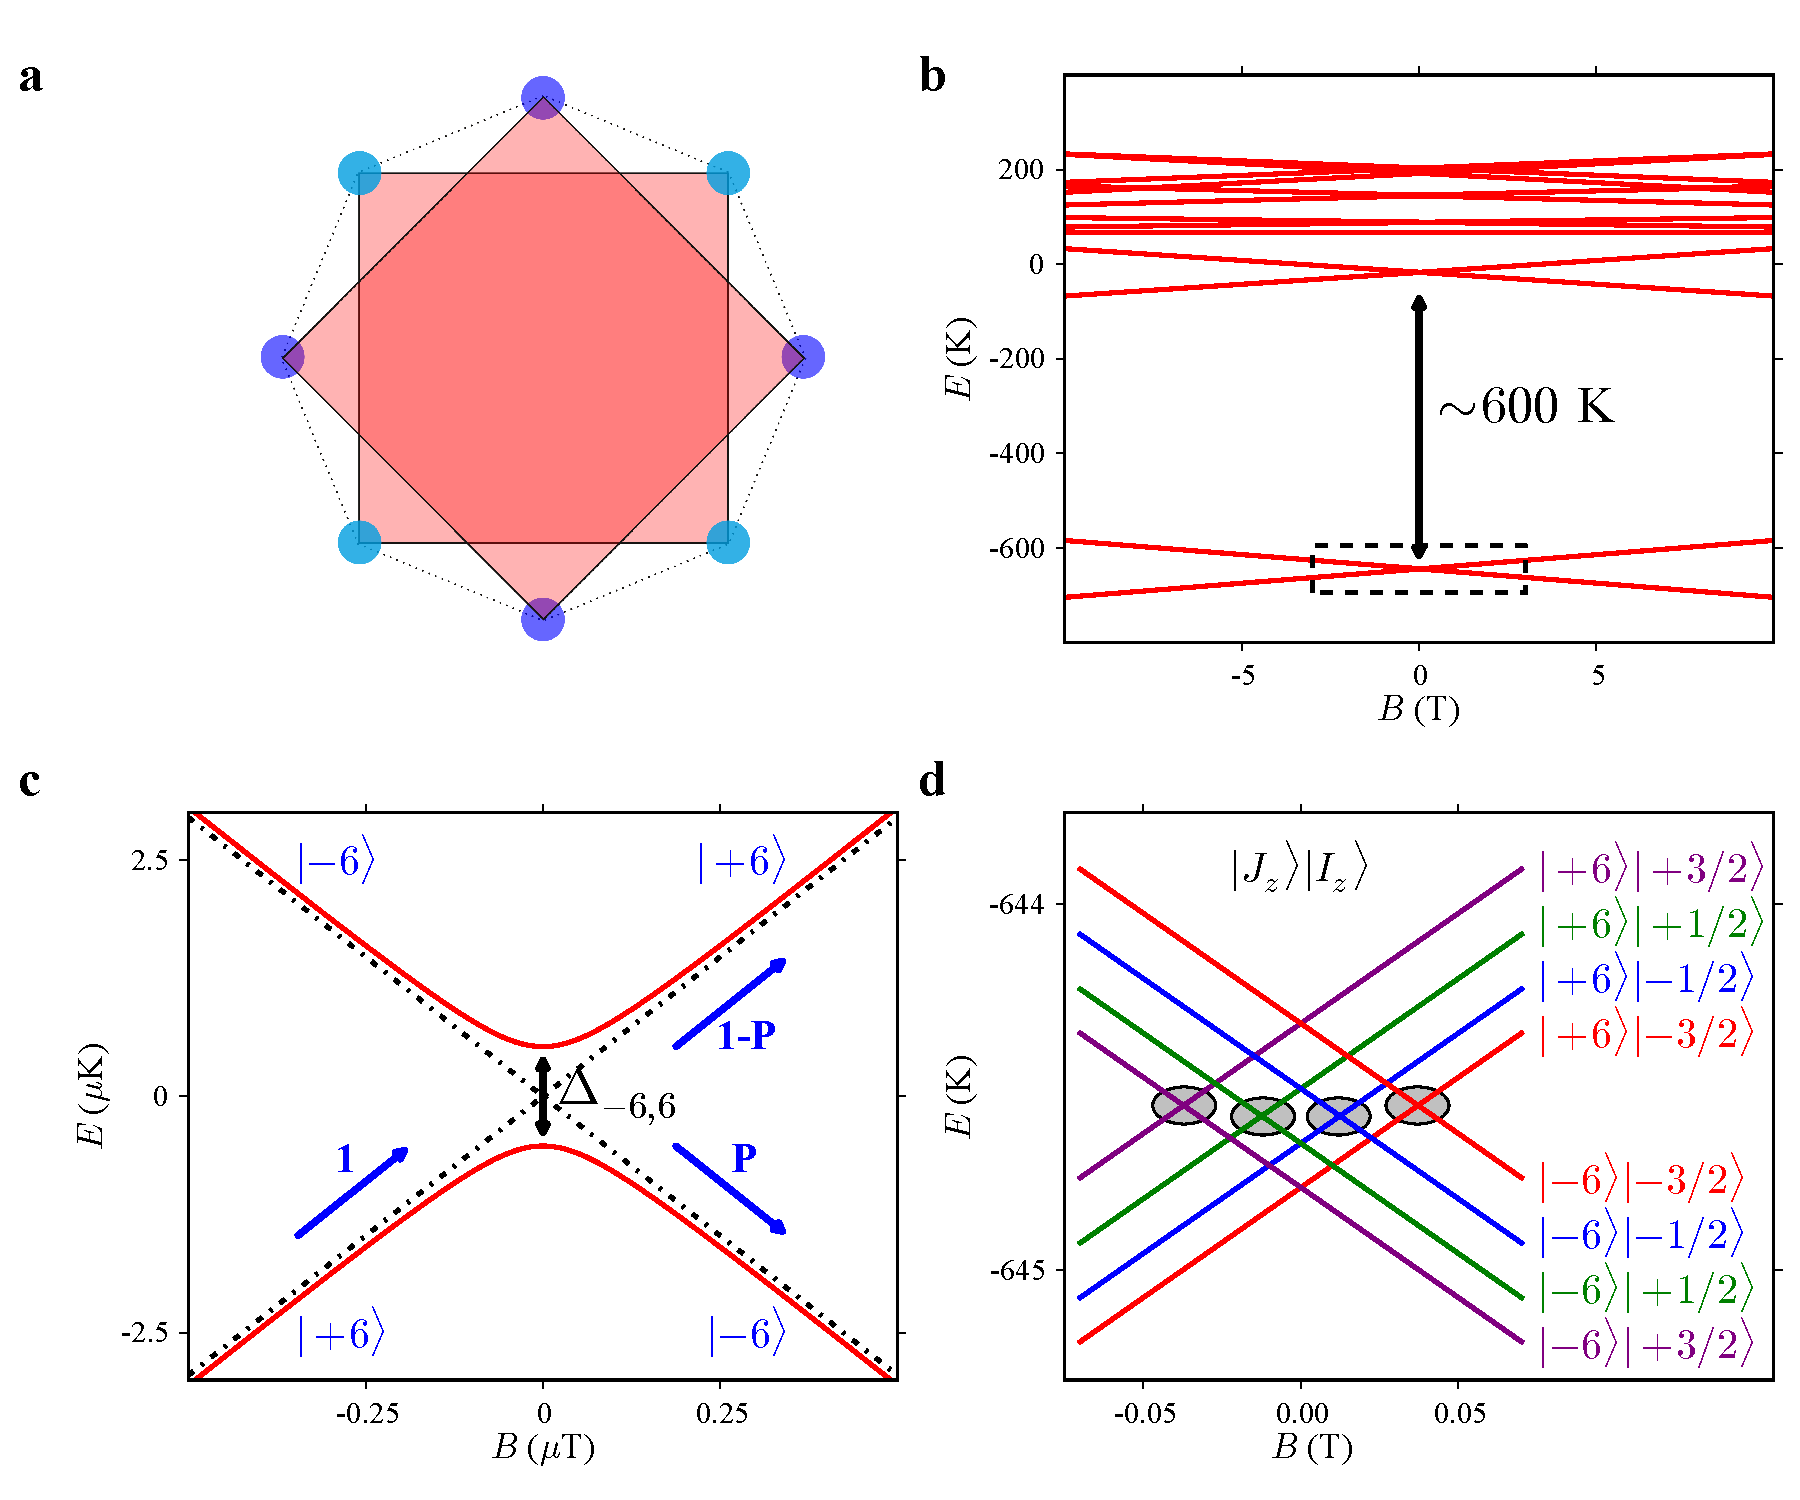
\includegraphics[scale=0.45]{Resultats/TbPc2Mag/TbPc2Mag.pdf} 
\caption{\textbf{a} : diagramme Zeeman de la molécule TbPc$_2$ représentant l'énergie des différents états du système en fonction du champ magnétique. Les états fondamentaux $J_z \pm 6$ sont séparés des premiers états excités par une énergie de $600$\,K. A basse température, on peut se concentrer sur les états fondamentaux. \textbf{b} : Agrandissement du diagramme Zeeman des deux états fondamentaux à faible champ magnétique. Il met en évidence un anti-croisement de valeur minimale $\Delta_{-6,6}$ de l'ordre du $\mu$K qui traduit une intrication entre les deux états.\textbf{c} : Diagramme Zeeman lorsque l'on tient compte du couplage hyperfin avec le spin $I=3/2$ du noyau. On ne relève que quatre anti-croisements marqués d'un cercle qui sont autant de zone ou les états $J_z =\pm6$ sont intriqués. \textbf{d} : Mesure de l'aimantation d'un cristal de TbPc$_2$ obtenu par technique micro-squid. Les molécules se retournent majoritairement à faible champ, ce qui correspond à quatre anti-croisements présentés dans \textbf{c}~(inspiré de \cite{Ishikawa2005}).}
\label{TbPc2Zeeman}
\end{figure}


\subsection{Hamiltonien}

\subsubsection{Le moment magnétique électronique}
L'ion terbium est lié de façon covalente à huit atomes d'azote, quatre pour chaque phatlocyanide. Les deux ligand sont orientés à $45\degres$ l'un par rapport à l'autre selon un axe perpendiculaire au plan des ligand. Cela correspond à une coordination dite anti-prisme~(cf Fig.\ref{TbPc2Imag}). De part cette configuration, le moment magnétique de l'ion terbium est soumis à un champ de ligand définie principalement par la longueur des liaisons covalentes et la symétrie du système. 

On peut rendre compte de ces différents paramètres en utilisant les opérateurs de Stevens. On obtient alors l'expression suivante :
\begin{eqnarray}
H = \alpha A_2^0 \langle r^2 \rangle O_2^0 + \beta A_4^0 \langle r^2 \rangle O_4^0 + \gamma A_6^0 \langle r^2 \rangle O_6^0
\end{eqnarray}
où les différents $O_i^0$ sont les opérateurs de Stevens, $A_i^0$ les coéfficients relatifs à la molécule de TbPc$_2$~\cite{Ishikawa2005} et $\alpha$, $\beta$ et $\gamma$ les coéfficients introduits par Stevens. Les opérateurs $O^0_i$ sont basés sur des sommes d'opérateurs $S_z^{2n}$. La symétrie du système n'introduit pas de couplage entre les différents états magnétiques. 

Le diagramme Zeeman correspondant est donné dans la Fig.\ref{TbPc2Zeeman}.a. Les états fondamentaux $J_z = \pm 6$ sont isolés des états excités par une énergie de plus de $600\,K$. Cela garantie, à basse température, deux états possibles pour le système : $J_z = \pm 6$. Dans la suite de notre description, on pourra négliger les états excités.

 
Cependant, du fait des interactions $\pi - \pi$ entre ligands, l'angle entre les deux plans n'est pas exactement égal à $45\degres$. Cela pour effet de briser la symétrie, ce qui nécessite l'introduction d'un nouveau terme dit terme transverse :
\begin{eqnarray}
H_{trans} = \beta A_4^4 \langle r^2 \rangle O_4^4
\end{eqnarray}
où la m\^eme notation a été utilisée. Ce dernier terme ne modifie pas l'allure générale du diagramme Zeeman. En revanche, il introduit un couplage entre les états  $J_z = \pm 6$ qui se traduit par la présence d'anti-croisement comme nous allons le voir maintenant.

\subsubsection{Les anti-croisements}
La Fig.\ref{TbPc2Zeeman}.b présente un grossissement du diagramme Zeeman au niveau de l'anti-croisement repréré par le carré en pointillé de la Fig.\ref{TbPc2Imag}.a. La ligne en pointillé correspond au diagramme Zeeman en l'absence de terme transverse. Si l'on se place loin de l'anti-croisement, les états $|+6\rangle$ et $|-6\rangle$ sont les états propre du système. Mais plus on se rapproche de l'anti-croisement, plus les états se mélangent.

Lorsque l'on balaie le champ magnétique autour d'un anti-croisement, il existe une probabilité de passer de l'état $|+6\rangle$ à l'état $|-6\rangle$ et vice-versas. Cette probabilité est régie par la formule de Landau-Zener~\cite{Zener1932} qui dépend à la fois de la séparation minimale entre les deux niveaux~$\Delta_{-6,6}$, ainsi que de la vitesse de balayage du champ magnétique~$\frac{dB_z}{dt}$. Cette probabilité peut s'exprimer de la façon suivante :
\begin{eqnarray}
P = 1 - \exp \left( -\frac{\pi \Delta^2_{m,m'}}{2 \hbar g \mu_B |m-m'|\frac{dB_z}{dt}} \right)
\end{eqnarray}
ou $P$ est la probabilité de passer de l'état $m$ à l'état $m'$, $m$ et $m'$ valant dans notre cas respectivement $+6$ et $-6$. Si la vitesse est très faible, la probabilité de passer d'un état à l'autre tend vers un. On retrouve ici le théorème adiabatique. A l'autre bout de l'échelle, si le champ magnétique est balayé très rapidement, cette probabilité tend vers zéro. Tout se passe comme si le système n'avait pas eu le temps de ``sentir" l'anti-croisement.




\subsubsection{Le spin nucléaire}
De part leur forme, les orbitales $4f$ impliquées dans le magnétisme du terbium, favorisent le couplage hyperfin. Il est donc possible de mesurer ce dernier dans les propriétés magnétiques de la molécule TbPc$_{2}$. Le spin nucléaire du terbium étant $I = 3/2$, on obtient en lieu et place des deux niveaux fondamentaux $J_z \pm 6$, deux jeux de quatre niveaux comme le montre la Fig.\ref{TbPc2Zeeman}.\textbf{c}. Cette interaction peut être prise en compte en introduisant le terme suivant dans l'hamiltonien :
\begin{eqnarray}
H_{hf} = A_{hf}\mathbf{J}\mathbf{I}
\end{eqnarray}
où $\mathbf{J}$ et $\mathbf{I}$ sont respectivement le moment magnétique électronique et le spin nucléaire, $A_{hf}$ étant la constante d'interaction hyperfine. Il est important de noter que le terbium ne possède qu'un seul isotope, et donc un seul spin nucléaire possible.

Du fait de sa forme allongée, le spin nucléaire possède également un moment quadripolaire dont on peut tenir compte en ajoutant le terme suivant à l'hamiltonien du système~\cite{Bleaney1961} :
\begin{eqnarray}
H_I = P\left(I_z^2 - \frac{1}{3}I(I+1)\right)
\end{eqnarray}
où $P$ est le moment quadripolaire du spin nucléaire. La présence de ce terme à pour conséquence de rendre l'espacement entre les différents niveaux non-uniforme. Ceci peut notamment avoir des applications dans le cadre de l'information quantique. Nous détaillerons ce dernier point plus tard, lorsque nous évoquerons les possibilités de manipulation du spin nucléaire.


\subsubsection{L'Hamiltonien de l'aimant moléculaire}

Ces différents terme doivent bien s\^ur \^etre inclus dans l'Hamiltonien total de l'aimant moléculaire. Cela donne, en reprenant la notion précédente :
\begin{eqnarray}
H = H_z + H_{//} + H_{\perp} + H_{hf} + H_I
\end{eqnarray}
Les trois derniers opérateurs agissent comme une perturbation et l'allure générale présenté dans la Fig.\ref{TbPc2Zeeman}.a n'est pas altéré. On peut donc continuer à ce concentrer sur les seuls états $J_z = \pm 6$. A cette échelle en revanche, les effets ne sont plus négligeables. En plus de l'anti-croisement introduit par la présence du plan difficile, le couplage hyperfin vient diviser les états fondamentaux  $J_z = \pm 6$ en deux jeux de quatre états, chacun de ces quatre états étant relatif à un état de spin nucléaire. De plus, pour un m\^eme état de spin nucléaire, l'anti-croisement entre les états de  $J_z = \pm 6$ est conservé. En revanche, seul des croisements sont observés pour les croisements entre les état de spins nucléaires différents~(cd Fig. \ref{TbPc2Zeeman}.c).


\subsection{Mesure de l'aimantation d'une assemblé}

Une mesure de l'aimantation d'un cristal de TbPc$_2$ pour différentes vittessses de balayage est présentée dans la Fig.\ref{TbPc2Zeeman}.d. Une analyse détaillée peut \^etre trouvé dans \cite{Ishikawa2005}. On peut diviser la courbe en deux zones. A faible champ, les molécules constituant le cristal se retournent par QTM. Les marches que l'on devine correspondent à la zone du diagramme Zeeman présentée dans la Fig.\ref{TbPc2Zeeman}.c et le retournement est gouverné par la formule de Landau-Zener. Il dépend donc de la vitesse ce qui conduit à une variation de la hauteur des marches en fonction de la vitesse de balayage. A plus fort champ, l'aimantation ne peut se retourner qu'en émettant un phonon d'où la zone de transition continue. L'influence de la vitesse de balayage n'est dans ce cas pas d\^u à un effet Landau-Zener mais à un effet que l'on nomme Phonon-Bottleneck. Il rend compte du fait qu'un trop grand nombre de molécules "souhaitent" se retourner pour que toutes puissent émettre un phonon.

\subsection{TbPc$_2$ et la spintronique}


\section{Mesure du retournement de l'aimantation}
\subsection{Transport à travers une boite quantique}
\subsection{Le couplage magnétisme-transport}
\subsubsection{Le couplage dipolaire}
\subsubsection{Le couplage d'échange}
\subsubsection{Le couplage magnéto-Coulomb}
\subsection{Le couplage mécanique}

\subsection{Intensité et nature de l'interaction}
\subsubsection{Amplitude des sauts de conductance}
\subsubsection{Intensité de l'interaction}

\subsection{Analyse des sauts en conductance}
\subsubsection{Méthode de détection}
\subsubsection{Interprétation physique de $\Delta g$}
\subsubsection{Choix du point de fonctionnement}
\subsubsection{Procédure d'alignement}

\subsection{Cycle d’hystérésis d'une assemblée versus une molécule isolé}
\subsubsection{A champ faible}
\subsubsection{A champ moyen}
\subsubsection{A champ fort}

\subsection{Dynamique du spin nucléaire}
\subsubsection{Temps de relaxation}
\subsubsection{Perturbations induites par la mesure}
\subsubsection{Influence de la tension de grille}
\subsubsection{Détermination de la température nucléaire}

\subsection{Perspectives}